\subsection{Erster Funktionstest} % (fold)
\label{sub:Erster Funktionstest}
\begin{frame}
\frametitle{Testsignalschaltung}
\framesubtitle{}
\begin{columns}[c]
    \column{0.65\textwidth}
         \begin{block}{$U_{in}$}
             \begin{itemize}
                \item $U_{in}$ liegt an Tiefpass:
                    \begin{equation*}
                        U_{in} = \frac{1}{\sqrt{\left(1+(R 2 \pi f
                        C)^2\right)}}\cdot U_{Fg} = 0.892V
                    \end{equation*}
                     für $f = 777Hz$,$U_{Fg} = 1V$
             \end{itemize}
         \end{block}
    \column{0.4\textwidth}
        \begin{figure}[H]
        \begin{center}
                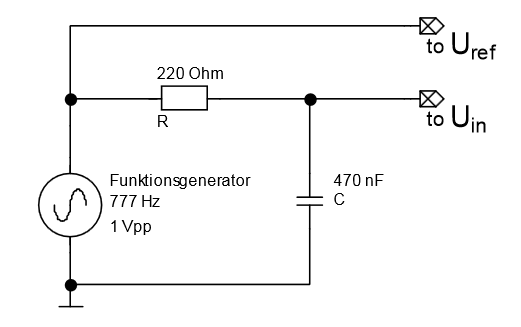
\includegraphics[scale=0.3]{./img/schaltung/testsignal.png}
        \end{center}
        \end{figure}
        \begin{figure}[H]
        \begin{center}
                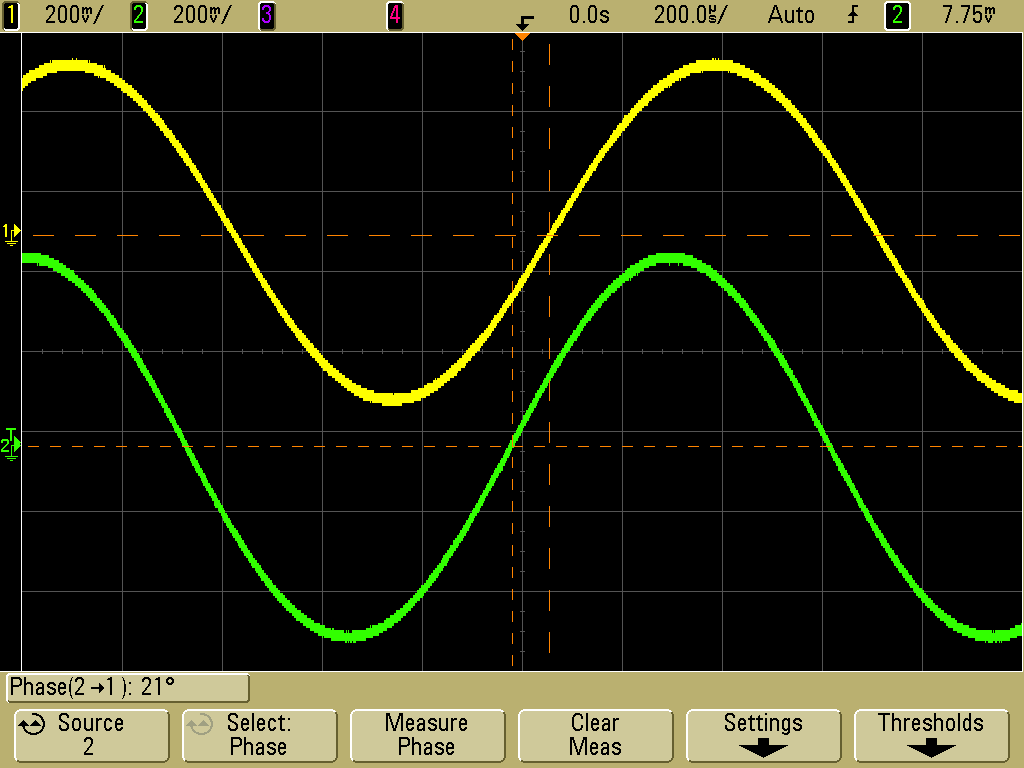
\includegraphics[scale=0.1]{./img/oszi/scope_21.png}
        \end{center}
        \end{figure}
        
        
\end{columns}

\end{frame}

\begin{frame}
\frametitle{Testsignalschaltung}
\framesubtitle{}
\begin{columns}[c]
    \column{0.65\textwidth}
         \begin{block}{Phase}
                 \begin{itemize}
                     \item Theoretische Phasenverschiebung:
                         \begin{equation*}
                             \varphi_{Th} = -\arctan{\left(2\pi f C R\right)} = 26.78^{\circ} 
                         \end{equation*}
                             für $f = 777Hz$
                    \item Gemessene Phasenverschiebung:
                        \begin{equation*}
                            \varphi_{Ge} = 21^{\circ}
                        \end{equation*}
                    \item
                        Mit $R_{Poti} = 6.96k\Omega$ bei maximalem $U_{out}$
                        ergibt sich eine Phasenverschiebung
                        \begin{equation*}
                            \varphi = 17.71^{\circ}
                        \end{equation*}
                 \end{itemize}
         \end{block}
    \column{0.4\textwidth}
        \begin{figure}[H]
        \begin{center}
                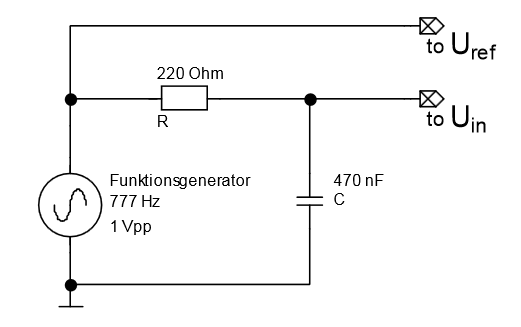
\includegraphics[scale=0.3]{./img/schaltung/testsignal.png}
        \end{center}
        \end{figure}
        \begin{figure}[H]
        \begin{center}
                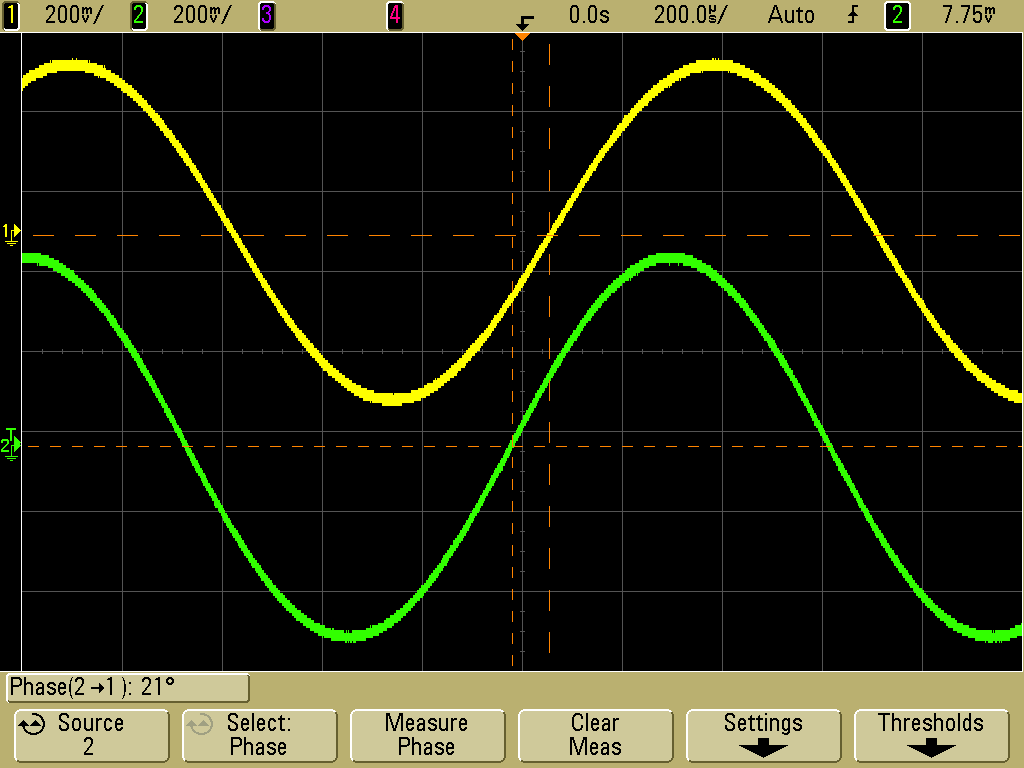
\includegraphics[scale=0.1]{./img/oszi/scope_21.png}
        \end{center}
        \end{figure}
\end{columns}
\end{frame}

\begin{frame}
    \frametitle{Messung}
    \framesubtitle{}
     \begin{figure}[H]
     \begin{center}
             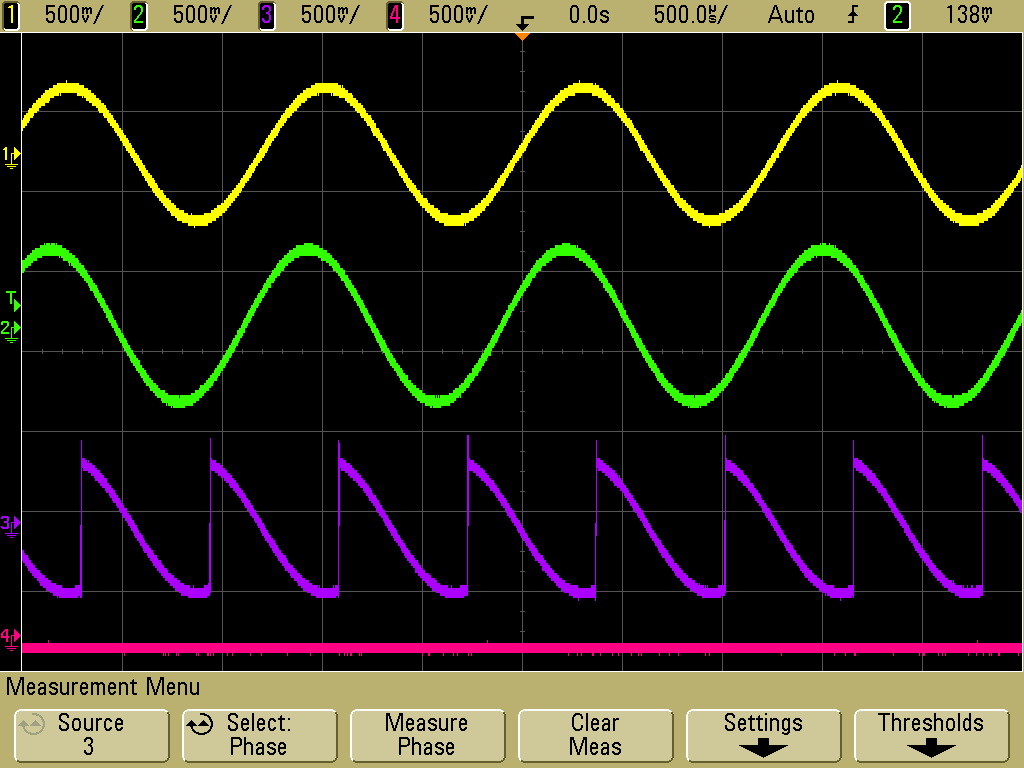
\includegraphics[scale=0.2]{./img/oszi/scope_18.png}
     \end{center}
     \caption{$U_{in}$ und $U_{ref}$ Phasenverschoben}
     \end{figure}
\end{frame}
\begin{frame}
    \frametitle{Messung}
    \framesubtitle{}
    \begin{figure}[H]
    \begin{center}
            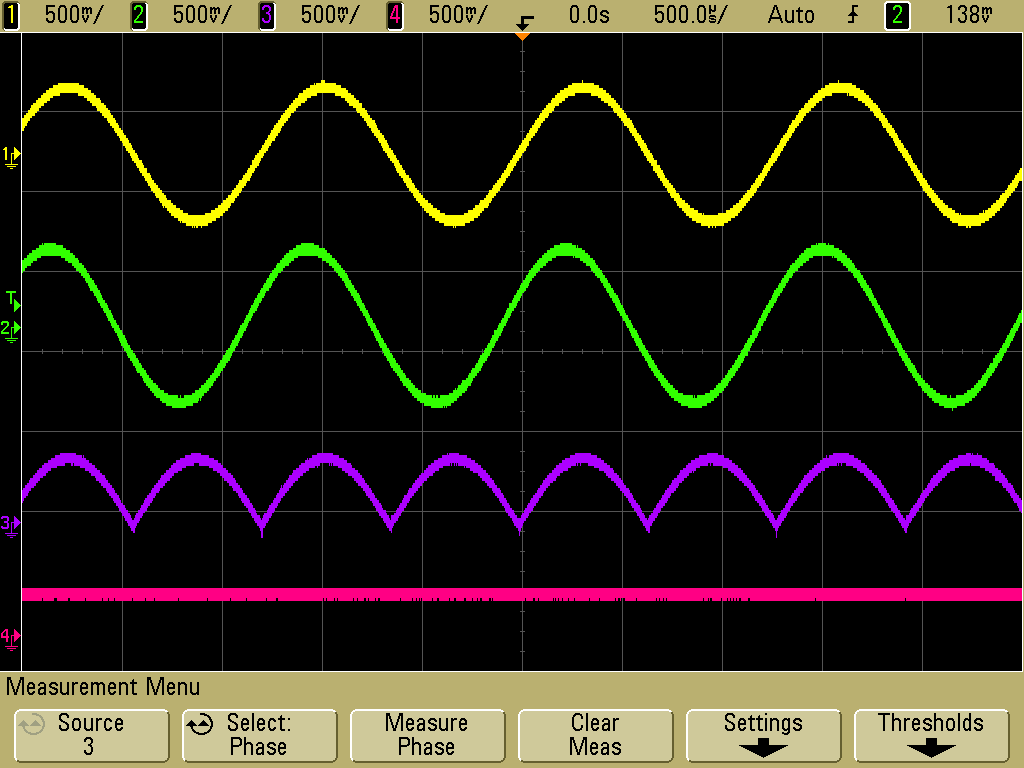
\includegraphics[scale=0.2]{./img/oszi/scope_17.png}
    \end{center}
     \caption{$U_{in}$ und $U_{ref}$ gleichphasig}
    \end{figure}
\end{frame}
% subsection Erster Funktionstest (end)
